\documentclass{article}

% If you do not have the 'neurips_2019' package specifically, 
% you can often use 'preprint' or standard article formatting. 
% Assuming the user has the style file provided in the prompt context:
\usepackage[final]{neurips_2019}

\usepackage[utf8]{inputenc}
\usepackage[T1]{fontenc}
\usepackage{hyperref}
\usepackage{url}
\usepackage{booktabs}
\usepackage{amsfonts}
\usepackage{nicefrac}
\usepackage{microtype}
\usepackage{graphicx}
\usepackage{xcolor}
\usepackage{amsmath} % Added for math environments
\usepackage{subcaption}
\usepackage{siunitx}
\usepackage{booktabs}  % for \toprule, \midrule, \bottomrule
\usepackage{multirow}  % for \multirow
\usepackage{tikz}
\usetikzlibrary{shapes,arrows,positioning,calc,fit}

\title{
  Active Characterization of Non-Cooperative Resident Space Objects Using Reinforcement Learning \\
  \vspace{1em}
  \small{\normalfont Stanford CS229 Project} 
}

\vspace{-40pt}

\author{
  Rahul Ayanampudi \\
  Department of Aeronautics and Astronautics \\
  Stanford University \\
  \texttt{rayanam@stanford.edu} \\
  \And
  Sebastian Martinez \\
  Department of Aeronautics and Astronautics \\
  Stanford University \\
  \texttt{sebasmp@stanford.edu}
}

\begin{document}
\maketitle
%\begin{abstract}
%Future missions for in-orbit servicing and active debris removal require autonomous spacecraft to characterize non-cooperative Resident Space Objects (RSOs) prior to proximity operations. This paper presents a reinforcement learning framework for active characterization, enabling a servicer spacecraft to autonomously plan maneuvers that maximize information gain regarding a target's 3D shape. We formulate the problem as a Partially Observable Markov Decision Process (POMDP) where the agent maintains a probabilistic voxel grid belief of the target. We implement a custom orbital dynamics simulator with a Monte Carlo Tree Search (MCTS) planner to guide exploration and generate training data for an AlphaZero-inspired policy network. Our results demonstrate that the standard MCTS planner effectively reduces belief entropy through optimized maneuver sequences, validating the approach for autonomous shape reconstruction in Low Earth Orbit (LEO) environments.
%\end{abstract}
\vspace{-30pt}
\section{Introduction}
The proliferation of space debris and the growing need for on-orbit servicing have made the autonomous characterization of Resident Space Objects (RSOs) a critical capability for future space missions. Before a servicer spacecraft can safely attempt docking or debris removal, it must fully characterize the target, a process that involves determining the relative orbit and reconstructing the target's 3D shape \citep{kruger2024adaptive}. Current observer systems largely rely on passive sensing, which suffers from range ambiguities and slow convergence rates due to a lack of geometric diversity in viewing angles.

To overcome these limitations, we propose an active sensing framework where the agent explicitly decides on maneuvers ($\Delta v$) to acquire the most informative observations. This problem presents significant challenges in several domains: orbital mechanics, guidance, navigation, and control (GNC), and computer vision. Furthermore, maneuvers that are optimal for orbit determination, such as those inducing parallax, are not necessarily optimal for shape reconstruction, which requires a diverse set of viewing angles to resolve occlusions. 

We model this problem as a POMDP. The input to our algorithm includes the fully observable physical state of the servicer relative to the target and the agent's internal belief state regarding the target's shape. The output is a discrete action representing an impulsive maneuver in the Radial-Tangential-Normal (RTN) frame. Training a policy that balances the cost of fuel expenditure against the information gain derived from reducing uncertainty in the target's volumetric model is done by leveraging an AlphaZero-style reinforcement learning architecture.

The problem formulation offers some advantages. First, impulsive spacecraft maneuvers naturally correspond to discrete actions, as thrusters execute finite-duration burns modeled as instantaneous velocity changes. Second, tree search can systematically evaluate possible maneuvers at each decision point \citep{kocsis2006bandit}, enabling principled long-horizon planning. This is critical for active sensing, where the information gain of future observations depends on selecting the right sequence of maneuvers.

\section{Related Work}
The challenge of autonomous spacecraft navigation has been extensively studied in the context of cooperative rendezvous. However, non-cooperative proximity operations introduce high uncertainty. \citet{kruger2024adaptive} proposed an adaptive end-to-end architecture for autonomous navigation, highlighting the necessity of robust estimation filters for proximity operations. Building on this, \citet{kruger2025autonomous} explored autonomous navigation using inter-satellite bearing angles, emphasizing the value of active maneuvering to improve observability in orbital regimes.

Our work draws inspiration from general reinforcement learning advancements in complex decision-making domains. Specifically, \citet{silver2017mastering} introduced the AlphaZero algorithm, which uses Monte Carlo Tree Search (MCTS) with a deep neural network to master games like Chess and Go without human domain knowledge. The goal is to adapt this "planning-and-learning" paradigm to the aerospace domain. 

The simulation utilizes Relative Orbital Elements (ROE), a geometric state representation developed by \cite{willis2023roe} that describes the relative motion trajectory. For the sensor model and belief update, we utilize the fast voxel traversal algorithm by \citet{amanatides1987fast} to efficiently simulate ray casting and occlusion in 3D space.

\section{Dataset and Simulation Environment}
We formulate active RSO characterization as a POMDP. The custom LEO simulator contains the servicer and the target RSO. The physical state ($s_{phys}$) of the servicer relative to the target (position and velocity) is assumed to be perfectly known to the agent. However, the true 3D shape of the target ($\mathcal{S}_{RSO_{shape}}$) is unknown and does not change with time. The agent's belief state $b_{{RSO}_{shape}}$ of the target is a probabilistic voxel grid where each cell $i$ contains a probability $P_i$ of being occupied. Initially, all cells are set to $P_i = 0.5$, representing maximum uncertainty. At the beginning of each episode, the relative orbital elements of the agent is initialized according to a random uniform Monte Carlo dispersion around a nominal scenario. The agent selects discrete impulsive maneuvers (13 actions: no-burn and $\pm \delta v_{\text{small}}, \pm \delta v_{\text{large}}$ along RTN axes) to minimize the entropy of its belief map while minimizing fuel expenditure.

The simulator propagates the ROE deterministically given an impulsive maneuver $\Delta v$. At each time step, the servicer captures an observation $o$ of the target with its 10$^\circ$ FOV, 64x64 resolution camera. The camera is assumed to always point at the center of the target and with optimal lighting conditions. We employ a ray-casting algorithm (3D DDA) to determine which voxels are visible from the current state \citep{amanatides1987fast}. The observation process includes sensor noise modeled within the likelihood function $P(o|\mathcal{S}, s_{phys})$. The agent calculates its own reward $R = \text{InfoGain} - \text{Cost}$. The $\text{Cost}$ comes from the action $a$, and the $\text{InfoGain}$ is calculated by the agent itself based on how the observation $o$ changed its internal belief. The projection of the camera observation of the orbiting servicer onto the probabilistic voxel grid enveloping the target is depicted in Figure \ref{voxel}.

\begin{figure}[h]
    \centering
    \includegraphics[width=0.45\linewidth]{figures/voxel.png}
    \caption{Probabilistic Voxel Belief Grid}
    \label{voxel}
\end{figure}

The dataset is generated dynamically in a self-play loop, as explained in Section \ref{section:rl-approach}. %In the execution phase, the agent uses the current neural network to guide a Monte Carlo Tree Search (MCTS), performing lookahead simulations to derive a robust policy distribution based on node visit counts. The agent then samples an action from this improved policy to propagate the spacecraft's orbital dynamics and update the belief grid, storing the time, initial state, action, reward, resulting state, and MCTS policy in a replay buffer. Finally, the neural network is trained on this collected data to minimize the error between its raw predictions and the superior MCTS policies and actual episode returns, creating a cycle of continuous improvement. 
    
\section{Methods}
Our approach uses Monte Carlo Tree Search (MCTS) as a classical planning algorithm to generate high-quality action sequences and compute target policies. Then, we adopt an AlphaZero-inspired self-play reinforcement learning framework where a neural network learns to approximate the planning results, enabling fast online decision-making.

\subsection{Reward Structure}
%The reward function is designed to incentivize the reduction of uncertainty in the voxel grid.
We quantify information gain using the reduction in Shannon entropy between time steps. The reward $R$ for a trajectory of length $T$ is defined as:
\begin{equation}
R = \sum_{t=0}^{T} \gamma^{t} \left[ \text{InfoGain}(b_{t}, b_{t+1}) - \lambda ||\Delta v_{a_{t}}|| \right]
\end{equation}
where $\text{InfoGain}$ corresponds to the decrease in total entropy of the probabilistic grid, and $\lambda$ is a weighting factor penalizing fuel consumption ($\Delta v$).

\subsection{Monte Carlo Tree Search (MCTS)} At each decision step, MCTS builds a search tree (Figure \ref{fig:MCTS_tree}) where nodes represent states and edges represent maneuvers.

\textbf{UCB1 Selection and Expansion:}
The tree search is guided by the Upper Confidence Bound (UCB1) formula, balancing exploitation of high-value actions with exploration of rarely visited states:
\begin{equation}
\text{UCB1}_i = Q(s,a_i) + c \sqrt{\frac{\ln N(s)}{N(s,a_i)}}
\end{equation}
where $c$ is the exploration constant, $Q(s,a_i)$ is the estimated mean return for action $a_i$ at state $s$, $N(s)$ is the total visits to state $s$, and $N(s,a_i)$ is the visits to action $a_i$ from $s$.
\textbf{Rollout Policy:}
At leaf nodes, the algorithm performs a rollout using a random rollout policy, where actions are sampled uniformly from the action space. This baseline approach provides a conservative estimate of future returns without domain-specific heuristics

\textbf{Backpropagation and Best Action Selection:}
After a fixed budget of iterations and tree depth, the best root action is selected greedily $a^* = \arg\max_i Q(s,a_i)$. The visit count distribution $\pi_{MCTS}(a|s) = N(s,a) / \sum_j N(s,a_j)$ represents an improved policy and serves as a training target for supervised learning.

\vspace{-20pt}
\subsection{Reinforcement Learning Framework}
\label{section:rl-approach}
An AlphaZero-inspired framework \citep{silver2018alphazero} is adopted, where a neural network learns to approximate the MCTS planning results through iterative self-play, alternating between two phases: (1) using MCTS guided by the current network to generate training data, and (2) training the network on the data to improve future planning. The observable state $s = (s_{phys}, b_{shape})$ consists of the ROE and the probabilistic voxel grid. The network processes these inputs through separate branches: 3D convolutions extract spatial features from the voxel grid, while fully-connected layers encode the ROE vector. After concatenation, a shared trunk outputs $f_{\theta}(s) = (\mathbf{p}, V_{\theta}(s))$, where the policy head produces $\pi_{\theta}(a|s) = \text{softmax}(\mathbf{p})$, action probabilities that guide tree search via the PUCT exploration bonus (Appendix \ref{appendix:PUCT}), and the value head outputs $V_{\theta}(s)$, predicting expected discounted return to bootstrap leaf node evaluations when confidence is sufficient. The neural network was programmed with PyTorch.

The training procedure is done in two phases. In the planning phase, starting from an initial state, MCTS with PUCT selection generates episodes by performing tree search at each step $t$. The policy network guides exploration toward promising actions, while the value network replaces expensive rollouts at leaf nodes when its confidence exceeds a threshold. After search completes at each step, we store the tuple $(s_t, \pi_{MCTS}(s_t), z_t)$ where $\pi_{MCTS} = N(s,a) / \sum_{a'} N(s,a')$ is the visit-count distribution and $z_t$ is the observed discounted return. Multiple episodes populate a replay buffer.

In the training phase, the network is updated by sampling mini-batches and minimizing $\mathcal{L}(\theta) = (z - V_{\theta}(s))^2 - \pi_{MCTS}(a|s)^{\top} \log \pi_{\theta}(a|s) + ||\theta||^2$, where the value loss trains the value head to predict returns, the policy loss trains the policy head to match MCTS policy via cross-entropy, and L2 regularization prevents overfitting. As the network improves, the expensive rollout simulations at leaf nodes are gradually replaced with fast network predictions $V_{\theta}(s_{leaf})$, which significantly accelerates MCTS planning in the self-play loop.

\subsection{Network Structure}
\begin{figure}[h]
\centering
\resizebox{\textwidth}{!}{%
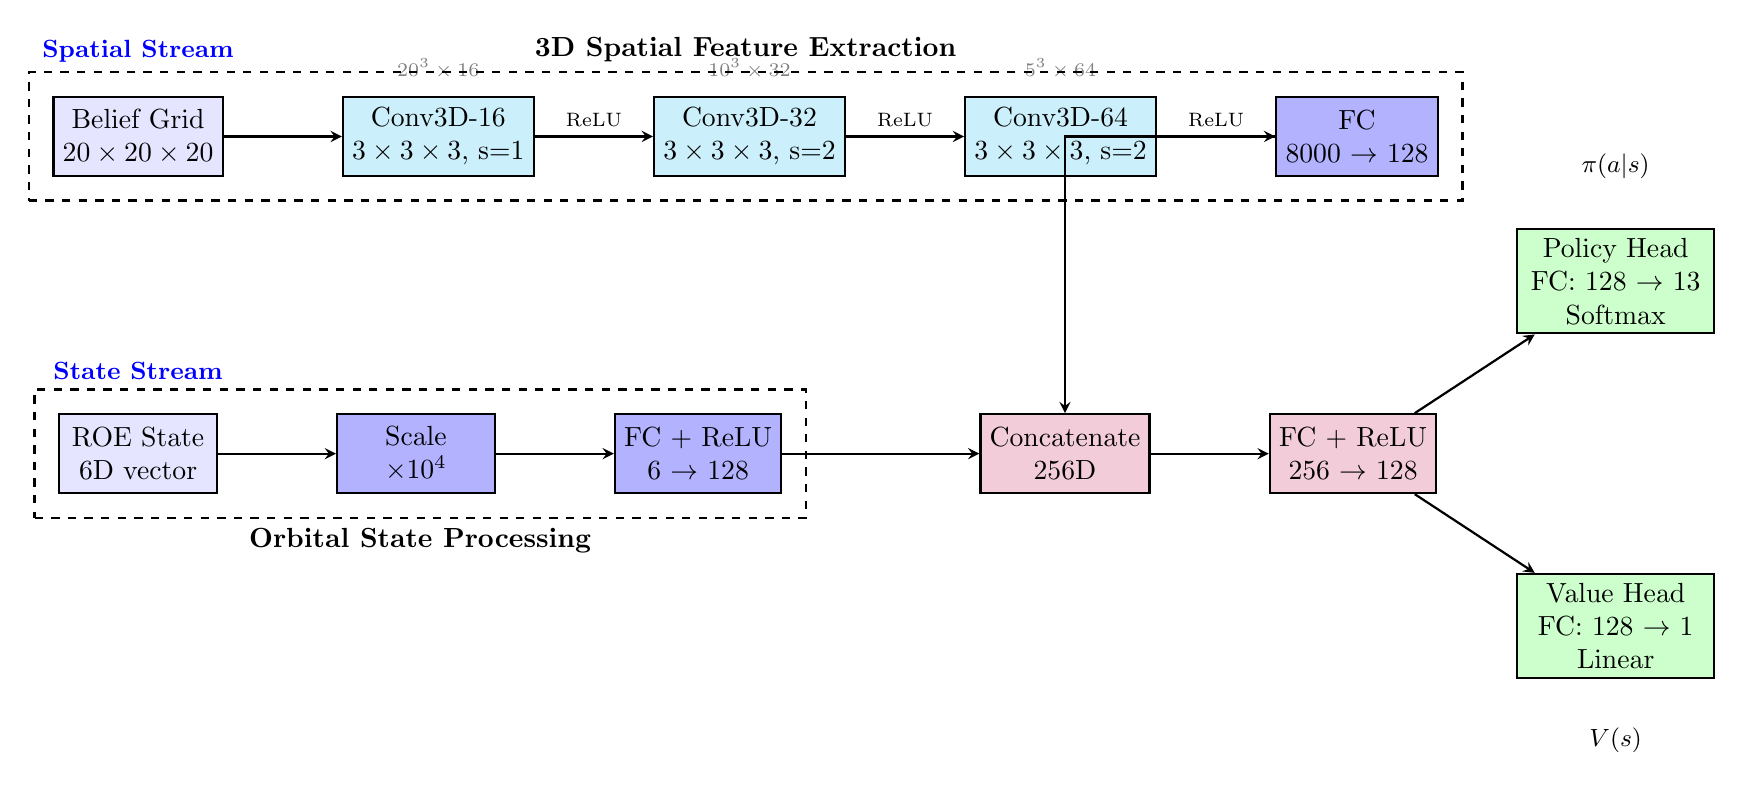
\begin{tikzpicture}[
    node distance=1.5cm,
    box/.style={rectangle, draw, thick, minimum width=2cm, minimum height=1cm, align=center},
    input/.style={box, fill=blue!10},
    conv/.style={box, fill=cyan!20},
    fc/.style={box, fill=blue!30},
    shared/.style={box, fill=purple!20},
    output/.style={box, fill=green!20, minimum width=2.5cm},
    arrow/.style={->, >=stealth, thick}
]

% Belief Grid Stream (Top)
\node[input] (grid_input) {Belief Grid\\$20 \times 20 \times 20$};
\node[conv, right=of grid_input] (conv1) {Conv3D-16\\$3 \times 3 \times 3$, s=1};
\node[conv, right=of conv1] (conv2) {Conv3D-32\\$3 \times 3 \times 3$, s=2};
\node[conv, right=of conv2] (conv3) {Conv3D-64\\$3 \times 3 \times 3$, s=2};
\node[fc, right=of conv3] (fc_grid) {FC\\8000 $\rightarrow$ 128};

% ROE Stream (Bottom)
\node[input, below=3cm of grid_input] (roe_input) {ROE State\\6D vector};
\node[fc, right=of roe_input] (scale) {Scale\\$\times 10^4$};
\node[fc, right=of scale] (fc_roe) {FC + ReLU\\6 $\rightarrow$ 128};

% Shared layers
\node[shared, right=2.5cm of fc_roe] (concat) {Concatenate\\256D};
\node[shared, right=of concat] (fc_shared) {FC + ReLU\\256 $\rightarrow$ 128};

% Output heads
\node[output, above right=1cm and 1cm of fc_shared] (policy) {Policy Head\\FC: 128 $\rightarrow$ 13\\Softmax};
\node[output, below right=1cm and 1cm of fc_shared] (value) {Value Head\\FC: 128 $\rightarrow$ 1\\Linear};

% Arrows - Grid stream
\draw[arrow] (grid_input) -- (conv1);
\draw[arrow] (conv1) -- node[above, font=\scriptsize] {ReLU} (conv2);
\draw[arrow] (conv2) -- node[above, font=\scriptsize] {ReLU} (conv3);
\draw[arrow] (conv3) -- node[above, font=\scriptsize] {ReLU} (fc_grid);

% Arrows - ROE stream
\draw[arrow] (roe_input) -- (scale);
\draw[arrow] (scale) -- (fc_roe);

% Arrows - Convergence
\draw[arrow] (fc_grid) -| (concat);
\draw[arrow] (fc_roe) -- (concat);
\draw[arrow] (concat) -- (fc_shared);

% Arrows - Output
\draw[arrow] (fc_shared) -- (policy);
\draw[arrow] (fc_shared) -- (value);

% Dimension annotations
\node[above=0.1cm of conv1, font=\scriptsize, text=gray] {$20^3 \times 16$};
\node[above=0.1cm of conv2, font=\scriptsize, text=gray] {$10^3 \times 32$};
\node[above=0.1cm of conv3, font=\scriptsize, text=gray] {$5^3 \times 64$};

% Stream labels
\node[above=0.3cm of grid_input, font=\small\bfseries, text=blue] {Spatial Stream};
\node[above=0.3cm of roe_input, font=\small\bfseries, text=blue] {State Stream};

% Final outputs
\node[above=0.5cm of policy, font=\small] {$\pi(a|s)$};
\node[below=0.5cm of value, font=\small] {$V(s)$};

% Add bounding boxes for clarity
\node[draw, dashed, thick, fit=(grid_input) (conv1) (conv2) (conv3) (fc_grid),
      label=above:{\textbf{3D Spatial Feature Extraction}}, inner sep=0.3cm] {};
\node[draw, dashed, thick, fit=(roe_input) (scale) (fc_roe),
      label=below:{\textbf{Orbital State Processing}}, inner sep=0.3cm] {};

\end{tikzpicture}
}
\caption{AlphaZero Policy-Value Network Architecture}
\label{fig:network_architecture}
\end{figure}

The network processes two input streams: a 3D voxel grid representing belief state (top) and a 6D ROE vector representing orbital state (bottom). After independent feature extraction, the streams are concatenated and processed through shared layers before splitting into policy and value heads for action selection and state evaluation.


\section{Experiments and Results}
%\subsection{Standard MCTS Planner}
%We conducted experiments to validate the efficacy of the MCTS planner in the orbital environment. The servicer was initialized in a standard inspection orbit relative to the target. The simulation parameters and justification for their values is provided in Appendix \ref{appendix:sim}.
%\subsubsection{Entropy Reduction}
%The primary metric for success is the reduction of belief entropy over time. Figure 1 (referencing the internal project figures) demonstrates the progression of total entropy over a 5-step episode. We observed a consistent monotonic decrease in entropy from an initial value of approximately 5550 nats to under 5000 nats. This confirms that the MCTS planner successfully selects maneuvers that reveal previously occluded faces of the RSO, thereby driving the voxel probabilities toward 0 (empty) or 1 (occupied).
%\subsubsection{Trajectory Analysis}
%Qualitative analysis of the trajectory shows that the agent does not simply drift passively. Instead, it executes burns that alter the relative geometry, specifically moving out of the orbital plane (Normal burns) to inspect the "top" and "bottom" of the target, which are typically unobservable in a planar fly-around. The visualization of the ray-casting interactions confirms that the agent prioritizes viewing angles that intersect with voxels holding high uncertainty ($P \approx 0.5$).
%\subsubsection{Discussion}
%The preliminary results indicate that the reward formulation effectively captures the objective of the mission. The trade-off between fuel cost and information gain prevents the agent from making prohibitively expensive maneuvers for marginal information return. While the current MCTS implementation serves as a strong baseline, the computational cost of running ray-casting simulations during the tree search is high. This justifies the proposed transition to the neural network policy, which will distill the MCTS capabilities into a fast forward-pass inference model suitable for real-time onboard deployment.
\subsubsection{MCTS Hyperparameter Tuning}

Hyperparameter sweeps were conducted to validate MCTS performance. The primary metrics are: (1) \textbf{Entropy Reduction (\%)}, measuring reconstruction completeness as $(H_{\text{initial}} - H_{\text{final}})/H_{\text{initial}} \times 100\%$, and (2) \textbf{Total $\Delta v$ (m/s)}, the cumulative fuel expenditure across the episode.

\paragraph{Experiment 1: Baseline Sweep (500 Iterations)}
Sweeps done over horizon $h \in \{10, 20\}$, exploration constant $c \in \{1.4, 2.0\}$, discount factor $\gamma \in \{0.9, 0.95, 0.99\}$, and fuel penalty $\lambda_{\Delta v} \in \{0.01, 0.1\}$. A total of 11 representative combinations were evaluated.

\begin{table}[h]
\centering
\caption{Experiment 1: Top 4 configurations by entropy reduction}
\begin{tabular}{cccccc}
\toprule
\textbf{c} & \textbf{h} & $\boldsymbol{\gamma}$ & $\boldsymbol{\lambda_{\Delta v}}$ & \textbf{Entropy Red. (\%)} & \textbf{Total $\Delta v$ (m/s)} \\
\midrule
1.4 & 20 & 0.99 & 0.010 & 96.60 & 0.75 \\
1.4 & 20 & 0.99 & 0.100 & 96.58 & 0.79 \\
1.4 & 10 & 0.95 & 0.010 & 73.52 & 0.71 \\
1.4 & 10 & 0.95 & 0.100 & 73.52 & 0.71 \\
\bottomrule
\end{tabular}
\label{tab:exp1_results}
\end{table}

Deeper planning ($h=20$, $\gamma=0.99$) achieves $\approx 97\%$ reconstruction with 0.75-0.79 m/s, while shallow planning ($h=10$, $\gamma=0.95$) achieves only 73.5\% with 0.71 m/s using the same exploration constant ($c=1.4$).

\paragraph{Experiment 2: Optimized Sweep (1000 Iterations)}
To test whether increased exploration can compensate for reduced planning depth, we fixed $h=10$ and $\gamma=0.99$ (high discount but shallow horizon), varying $c \in \{1.4, 2.0, 3.0\}$ and $\lambda_{\Delta v} \in \{0.5, 1.0, 5.0\}$ with 1000 MCTS iterations.

\begin{table}[h]
\centering
\caption{Experiment 2: Configurations ranked by entropy reduction}
\begin{tabular}{cccc}
\toprule
\textbf{c} & $\boldsymbol{\lambda_{\Delta v}}$ & \textbf{Entropy Red. (\%)} & \textbf{Total $\Delta v$ (m/s)} \\
\midrule
3.0 & 0.5 & 96.37 & 1.10 \\
3.0 & 1.0 & 94.96 & 1.17 \\
1.4 & 1.0 & 94.60 & 1.36 \\
2.0 & 1.0 & 93.39 & 1.40 \\
\bottomrule
\end{tabular}
\label{tab:exp2_results}
\end{table}

Aggressive exploration ($c=3.0$) with increased computational budget recovers near-optimal performance (96.37\%) despite shallow planning, demonstrating that exploration breadth can compensate for reduced lookahead depth. However, this requires 47\% more fuel (1.10 vs 0.75 m/s) than Experiment 1's deep planning approach.

\paragraph{Key Insights}
%The experiments reveal a fundamental tradeoff between planning depth and exploration breadth. Deep planning ($h=20$) achieves $\approx 97\%$ reconstruction with moderate exploration ($c=1.4$) using only 0.75 m/s, while shallow planning ($h=10$) requires aggressive exploration ($c=3.0$) and 1000 iterations to achieve similar reconstruction (96.37\%) but consumes 47\% more fuel (1.10 m/s). This demonstrates that lookahead depth is more fuel-efficient than exploration breadth for active sensing in orbital domains. Fuel penalty $\lambda$ must be carefully tuned: excessively high values ($\lambda \geq 5.0$) degrade performance, while moderate values ($\lambda \leq 1.0$) enable $>90\%$ reconstruction. The best overall configuration ($c=1.4$, $h=20$, $\gamma=0.99$, $\lambda=0.01$, 500 iterations) achieves 96.60\% entropy reduction with 0.75 m/s, validating MCTS as an effective baseline for fuel-constrained active sensing.

Experiments reveal a fundamental tradeoff between planning depth and exploration breadth. Deep planning ($h=20$) achieves $\approx 97\%$ reconstruction using only 0.75 m/s, while shallow planning ($h=10$) requires aggressive exploration and 1000 iterations to achieve similar performance (96.37\%) but consumes 47\% more fuel (1.10 m/s), demonstrating that lookahead depth is more fuel-efficient than exploration breadth. The best configuration ($c=1.4$, $h=20$, $\gamma=0.99$, $\lambda=0.01$) achieves 96.60\% entropy reduction with 0.75 m/s.

\subsection{AlphaZero MCTS Planner}

\subsubsection{Simulation Parameters and Neural Network Hyperparameter Tuning}
The AlphaZero MCTS planner hyperparameters were tuned with sweeps similar to the top performing configuration for pure MCTS. Tables \ref{tab:training_config} and \ref{tab:env_config} exhibit a parameter configuration that balances four key considerations: physical realism, computational tractability, learning complexity, and adherence to standard hyperparameter conventions.

After each batch of self-play episodes, the network undergoes 5 training epochs to prevent underfitting while avoiding excessive optimization on a single data batch. The replay buffer maintains 20,000 transitions (approximately 6 full episodes), providing sample diversity for decorrelating batches while keeping the training distribution relatively on-policy.
\begin{table}[htbp]
    \centering
    %--- First Table (Left) ---
    \begin{minipage}[t]{0.48\textwidth}
        \centering
        \caption{Environment Configuration}
        \label{tab:env_config}
        \small
        \resizebox{\textwidth}{!}{% Optional: Resizes table to fit width exactly
        \begin{tabular}{llr}
            \toprule
            \textbf{Category} & \textbf{Parameter} & \textbf{Value} \\
            \midrule
            \multirow{4}{*}{Simulation}
              & Max Horizon & 5 \\
              & Num Steps & 50 \\
              & Time Step (s) & 120.0 \\
              & Num Episodes & 130 \\
            \midrule
            \multirow{5}{*}{Orbit}
              & $\mu_{\text{Earth}}$ (km$^3$/s$^2$) & 398600.4 \\
              & Semi-major $a_{\text{chief}}$ & 7000.0 \\
              & Eccentricity $e_{\text{chief}}$ & 0.001 \\
              & Inclination $i_{\text{chief}}$ & 98.0$^{\circ}$ \\
              & RAAN $\Omega_{\text{chief}}$ & 30.0$^{\circ}$ \\
            \midrule
            \multirow{6}{*}{\shortstack[l]{Initial ROE\\(Nominal\\$\pm$ Bounds)\\$[m]$}}
              & $\delta a$ & $0 \pm 0$ \\
              & $\delta \lambda$ & $200 \pm 20$ \\
              & $\delta e_x$ & $100 \pm 10$ \\
              & $\delta e_y$ & $0 \pm 10$ \\
              & $\delta i_x$ & $50 \pm 10$ \\
              & $\delta i_y$ & $0 \pm 10$ \\
            \bottomrule
        \end{tabular}
        }
    \end{minipage}
    \hfill % Adds flexible space between the tables
    %--- Second Table (Right) ---
    \begin{minipage}[t]{0.48\textwidth}
        \centering
        \caption{Hyperparameters}
        \label{tab:training_config}
        \small
        \resizebox{\textwidth}{!}{% Optional: Resizes table to fit width exactly
        \begin{tabular}{llr}
            \toprule
            \textbf{Category} & \textbf{Parameter} & \textbf{Value} \\
            \midrule
            \multirow{12}{*}{\shortstack[l]{AlphaZero\\Training}}
              & Batch Size & 64 \\
              & Learning Rate & $5 \text{e-}4$ \\
              & MCTS Iterations & 100 \\
              & Epochs/Cycle & 5 \\
              & Replay Buffer & 20000 \\
              & $c_{\text{PUCT}}$ & 1.4 \\
              & Discount $\gamma$ & 0.99 \\
              & Weight Decay & $1 \text{e-}4$ \\
              & Grad Clip Norm & 1.0 \\
              & Optimizer & Adam \\
              & Scheduler & Cosine \\
              & Min LR & $1 \text{e-}5$ \\
            \midrule
            \multirow{1}{*}{Control}
              & $\lambda_{\Delta v}$ (penalty) & 1.0 \\
            \bottomrule
        \end{tabular}
        }
    \end{minipage}
\end{table}

\subsubsection{AlphaZero MCTS Performance}
\begin{figure*}[h]
    \centering
    \begin{subfigure}[t]{0.5\textwidth}
        \centering
        \includegraphics[height=2.2in]{figures/alphazero_mcts_orbit.png}
        \caption{AlphaZero MCTS Agent Orbit}
        \label{fig:AlphaZero_MCTS_Orbit}
    \end{subfigure}%
    ~ 
    \begin{subfigure}[t]{0.5\textwidth}
        \centering
        \includegraphics[height=2.2in]{figures/baseline_final_frame.png}
        \caption{Passive Agent Orbit Baseline: No Burns}
        \label{fig:passive}
    \end{subfigure}
    \caption{AlphaZero MCTS and Baseline Orbit Comparison}
    \label{output_traj_comparsion}
\end{figure*}

The trained AlphaZero MCTS agent was tested in the simulation and compared against the standard MCTS planner and the no-burn baseline. Figure \ref{output_traj_comparsion} depicts the servicer orbiting around the target, performing burns, and taking camera observations. As exhibited, the AlphaZero MCTS planner successfully outperforms the passive agent by taking only 3 small maneuvers ($\Delta v =$ \SI{0.11}{\frac{\meter}{\second}}) out of the 50 time steps, decreasing the entropy by approximately 97.1\% of the agent's initial entropy and beating the baseline by 1.3\%. For reference, the standard MCTS implementation yielded an entropy reduction improvement of approximately 0.23\% with $\Delta v =$ \SI{0.24}{\frac{\meter}{\second}} with respect to the baseline. Given that the $\Delta v$ budget of current small passive observer satellites is on the order of \SI{10}{\frac{\meter}{\second}} for basic station-keeping, both the standard MCTS and AlphaZero MCTS planners provide a reasonable trajectory that boosts performance. The experiment results clearly demonstrate that the active characterization enabled by the AlphaZero MCTS planner represents a significant advancement over traditional passive observers. 

\begin{figure*}[h]
    \centering
    \begin{subfigure}[t]{0.5\textwidth}
        \centering
        \includegraphics[height=1.55in]{figures/value_loss.png}
        \caption{Value Loss}
        \label{fig:val}
    \end{subfigure}%
    ~ 
    \begin{subfigure}[t]{0.5\textwidth}
        \centering
        \includegraphics[height=1.55in]{figures/policy_loss.png}
        \caption{Policy Loss}
        \label{fig:pol}
    \end{subfigure}
    \caption{AlphaZero MCTS Network Losses}
    \label{loss}
\end{figure*}

As shown in Figure \ref{loss}, the value network demonstrated strong learning with a 89\% reduction in loss, while the policy network remained essentially stagnant with minimal variance early in the training and decreased from there. This rapid convergence suggests the model may have settled into a local optimum early, as the total loss improvement was driven almost entirely by better value predictions rather than refined action strategies. To address this policy stagnation, future runs will adjust hyperparameters such as the network learning rate, MCTS iterations, or the exploration constant to encourage broader state-space exploration. 

\section{Conclusion and Future Work}
We have presented a framework for active characterization of around non-cooperative RSO using reinforcement learning. By modeling the problem as a POMDP and utilizing AlphaZero MCTS over a probabilistic voxel grid, we demonstrated that an autonomous agent can plan maneuvers that significantly reduce shape uncertainty. The results validate the use of AlphaZero MCTS in orbital proximity operations as it successfully outperformed the passive agent with minimal $\Delta v =$ \SI{0.11}{\frac{\meter}{\second}} by decreasing the entropy by approximately 97.1\% of the agent's initial entropy. The fact that it beat the baseline proves it has learned to manipulate the orbit geometry to its advantage. This improvement could be the differentiating factor that leads to a successful mission.

Future work will focus on further training of the AlphaZero MCTS planner. This involves generating a large-scale dataset of self-play episodes to train the policy and value networks, thereby replacing the expensive MCTS rollout phase at runtime. Additionally, we plan to increase the fidelity of the simulation by introducing realistic guidance, navigation, and control errors and solar lighting conditions to challenge the robustness of the vision system. Prior to industry adoption, a safety validation algorithm such as reachability analysis to check for collisions prior to burn execution would be introduced. With these refinements, the, planner will be able to make smart maneuvers, react to lighting conditions, drift, or occlusions, and be able to correct a suboptimal initial orbit, shaping AlphaZero MCTS to be a powerful tool for active characterization of non-cooperative RSO and providing capabilities that far surpass current systems on the market.

\section{Appendices}

\subsection*{Simulation Parameter Justification Summary}

\begin{itemize}
    \item \textbf{Simulation}: 50-step episodes with $\Delta t = \SI{120}{\second}$ span approximately one orbit. MCTS horizon of 5 balances lookahead with computational cost.

    \item \textbf{Orbit}: \SI{7000}{\kilo\meter} LEO sun-synchronous orbit ($i = \SI{98}{\degree}$, $e = 0.001$) represents typical Earth observation missions (consistent lighting) with near-circular trajectories.

    \item \textbf{Camera}: \SI{10}{\degree} FOV and $64 \times 64$ resolution match embedded satellite constraints; asymmetric noise model ($P(\text{hit}|\text{occ}) = 0.95$, $P(\text{hit}|\text{emp}) = 0.001$) enforces partial observability.

    \item \textbf{Initial ROE}: Nominal $\delta \lambda = \SI{200}{\meter}$, $\delta e_x = \SI{100}{\meter}$, $\delta i_x = \SI{50}{\meter}$ with $\pm$10--20~m perturbations across 65 episodes tests generalization.

    \item \textbf{Monte Carlo Perturbations}: The expensive computations limited the number of episodes that could be run. However, the AlphaZero MCTS approach has high sample efficiency and accuracy since the network provides a high-quality evaluation based on pattern recognition from training. It essentially gives the MCTS "intuition," making the value estimates ($Q$-values) much closer to the ground truth (optimal play). Hence, the AlphaZero MCTS planner needs fewer episodes to yield a good policy. The perturbation magnitudes were chosen based on domain knowledge.

    \item \textbf{Network}: 128 hidden units and $20^3$ voxel grid balance expressiveness with computational tractability. 13 discrete actions enable MCTS search.

    \item \textbf{Control}: $\lambda_{\Delta v} = 1.0$ provides equal weighting of entropy reduction and fuel cost.
\end{itemize}

The training process employs a batch size of 64 samples, providing stable gradient estimates while fitting within typical memory constraints. The Adam optimizer uses an initial learning rate of $5 \times 10^{-4}$, a conservative value that prevents catastrophic forgetting in the continual learning setting while allowing effective policy updates. This learning rate is gradually reduced via cosine annealing to a minimum of $1 \times 10^{-5}$ over the training duration, enabling fine-tuning without completely halting adaptation to new data. Weight decay regularization ($\lambda = 1 \times 10^{-4}$) and gradient clipping (max norm = 1.0) provide additional stability and prevent overfitting to specific trajectories.

Each MCTS search performs 100 iterations, balancing search quality with computational cost (approximately 1--2 seconds per search on modern CPUs) and exploring roughly 10 actions to depth 2--3. The exploration constant $c_{\text{PUCT}} = 1.4$ follows the standard AlphaZero formulation, balancing exploitation of promising moves with exploration of unvisited nodes. After each batch of self-play episodes, the network undergoes 5 training epochs to prevent underfitting while avoiding excessive optimization on a single data batch. The replay buffer maintains 20,000 transitions (approximately 6 full episodes), providing sample diversity for decorrelating batches while keeping the training distribution relatively on-policy.

The discount factor $\gamma = 0.99$ appropriately weights long-term rewards for the 50-step episodes ($\gamma^{50} \approx 0.605$), ensuring that terminal rewards significantly influence early-episode decisions while preventing the myopic behavior that would result from lower discount factors. The fuel cost penalty $\lambda_{\Delta v} = 1.0$ provides equal weighting between information gain (entropy reduction) and fuel consumption in the reward function, establishing a neutral baseline for subsequent tuning studies.

The configuration strikes a balance between physical realism (orbital mechanics, sensor models), computational constraints (training time, memory), and learning theory (exploration, generalization, stability).

\subsection{MCTS}
\subsubsection{MCTS Tree Example}
\begin{figure*}[h]
    \centering
    \includegraphics[width=\textwidth]{figures/mcts_tree_example.png}
    \caption{MCTS Tree of Depth 2}
    \label{fig:MCTS_tree}
\end{figure*}

\subsubsection{PUCT Selection}
\label{appendix:PUCT}
An enhancement from AlphaZero is the use of the Polynomial Upper Confidence Trees (PUCT) formula for action selection during tree search, which directly incorporates the neural network's policy prior. During tree traversal, actions are selected according to:
\begin{equation}
a^* = \arg\max_a \left[ Q(s,a) + c \cdot \pi_{\theta}(a|s) \cdot \frac{\sqrt{N(s)}}{1 + N(s,a)} \right]
\end{equation}
where $\pi_{\theta}(a|s)$ is the policy network's predicted probability for action $a$. This modification allows the network to guide exploration toward promising actions earlier in the search, improving sample efficiency. When the network is untrained or not available, the system falls back to standard UCB1.

\subsubsection{Entropy Progression} \label{appendix:entropy}
Each episode of the simulation has a non-increasing entropy progression plot. However, some runs have more entropy reduction than others. An example of an AlphaZero MCTS episode entopy progression is shown in Figure \ref{fig:entropy}.

\begin{figure}[h]
    \centering
    \includegraphics[width=0.45\linewidth]{figures/entropy.png}
    \caption{AlphaZero MCTS Episode Entropy Progression Example}
    \label{fig:entropy}
\end{figure}

\subsubsection{Policy and Value Network Loss} \label{appendix:loss}
Although there is no trivial baseline to compare the network loss to, the policy and value loss decrease and plateau below the threshold. Initially, when the network knows nothing, it assigns equal probability ($1/13$) to every action, making the cross entropy loss $-ln(\frac{1}{13}) = 2.5649$. As shown in Figure \ref{fig:loss}, the policy loss decreases from the random policy loss and the value loss decreases, as expected.

% \begin{figure}[h]
%     \centering
%     \includegraphics[width=0.45\linewidth]{figures/loss.png}
%     \caption{AlphaZero MCTS Network Policy Loss}
%     \label{fig:loss}
% \end{figure}

\subsection{Hardware}
The parallelized simulation episodes with 13 workers and network training was performed on an Intel Core i7 processor. The training time for a single batch of 13 episodes with the parameters listed in Tables \ref{tab:training_config} and \ref{tab:env_config} was approximately 6 hours. The largest bottleneck is the expensive ray tracing with 64x64 sensor resolution. Adjusting the maximum iterations, horizon, number of simulation time steps, and number of episodes also directly affect runtime.

\section{Contributions}
\textbf{Rahul Ayanampudi}: Developed the relative orbital dynamics simulator. Defined the POMDP state/action spaces, probabilistic voxel grid belief, ray-casting sensor observation model, and reward function. Structured the neural network, parallelized episodes, and trained the network.

\textbf{Sebastian Martinez}: Configured the reinforcement learning problem formulation. Implemented the standard MCTS logic, integrated the planning algorithm with the environment, and performed hyperparameter tuning. Created the AlphaZero-inspired MCTS framework.

The Github repository can be found in \href{https://github.com/rayanam2021/CS229_Final_Project}{https://github.com/rayanam2021/CS229\_Final\_Project}

\bibliographystyle{plainnat}
\bibliography{references}

\end{document}